% !TeX root = ../Harte_Kugeln.tex
\subsection{Paarverteilungsfunktion}
Eine Flüssigkeit oder ein Gas mit rein additiven Paarwechselwirkungen kann durch die sogenannte Paarverteilungsfunktion --- manchmal auch Paarkorrelationsfunktion oder radiale Verteilungsfunktion --- $g(r)$ vollständig charakterisiert werden. Diese Funktion gibt Aufschluss über die kurzreichweitige Struktur des Fluids --- also seine Nahordnung. Sie beschreibt die Häufigkeit, mit der sich zwei Teilchen in einem gewissen Abstand $r$ voneinander entfernt befinden, bezogen auf die jeweilige Häufigkeit in einem idealen Gas. Die Paarverteilungsfunktion ist demnach gegeben durch
\begin{equation}
g(r) = \frac{1}{4\pi r^2 \rho} \langle \sum_{j\neq i} \delta(r-r_{ij}) \rangle
\end{equation}   
Da Fluide keine Fernordnung besitzen, muss die Paarverteilungsfunktion im limes $r \rightarrow \infty$ gegen 1 konvergieren. Des weiteren sei angemerkt, dass die Paarverteilungsfunktion der Randverteilung der $N$-Teilchen-Wahrscheinlichkeitsdichte entspricht und man demnach im limes $\rho \rightarrow 0$ direkt das Paarpotential $U(r)$ aus der Paarverteilungsfunktion ablesen kann.  
\begin{equation}
\lim_{\rho \rightarrow 0} g(r) = e^{-\beta U(r)}
\end{equation}
Für Festkörper lässt sich natürlich auch eine Paarverteilungsfunktion definieren, allerdings ist diese nicht mehr isotrop sondern richtungsabhängig. 
\begin{equation}
g(\vec{r}) = \frac{1}{\rho N} \langle \sum_{j\neq i} \delta^{(3)}(\vec{r}-\vec{r_{ij}}) \rangle
\end{equation} 
Häufig wird aber auch die winkelgemittelte Version verwendet, welche dann mit der Definition der Paarverteilungsfunktion für Fluide übereinstimmt. 

Abbildungen \ref{fig:paarverteilung1}, \ref{fig:paarverteilung2} und \ref{fig:paarverteilung3} zeigen die Paarverteilungsfunktionen des Systems von Harte Kugeln für verschiedene Dichten $\rho$ von 0.2 bis 1.3. Die Entstehung von Nahordnung beim Übergang vom gasförmigen zum flüssigen Zustand mit zunehmender Dichte lässt sich gut anhand von Abbildung \ref{fig:paarverteilung1} erkennen. Im ungeordneten (gasförmigen) Zustand nimmt die Paarverteilungsfunktion mit der Entfernung monoton ab, während sich beim Phasenübergang zur Flüssigkeit ein zweites Maximum ausbildet. 
\begin{figure}[H]
 \centering
 \resizebox{0.9\textwidth}{!}{% GNUPLOT: LaTeX picture with Postscript
\begingroup
  \makeatletter
  \providecommand\color[2][]{%
    \GenericError{(gnuplot) \space\space\space\@spaces}{%
      Package color not loaded in conjunction with
      terminal option `colourtext'%
    }{See the gnuplot documentation for explanation.%
    }{Either use 'blacktext' in gnuplot or load the package
      color.sty in LaTeX.}%
    \renewcommand\color[2][]{}%
  }%
  \providecommand\includegraphics[2][]{%
    \GenericError{(gnuplot) \space\space\space\@spaces}{%
      Package graphicx or graphics not loaded%
    }{See the gnuplot documentation for explanation.%
    }{The gnuplot epslatex terminal needs graphicx.sty or graphics.sty.}%
    \renewcommand\includegraphics[2][]{}%
  }%
  \providecommand\rotatebox[2]{#2}%
  \@ifundefined{ifGPcolor}{%
    \newif\ifGPcolor
    \GPcolortrue
  }{}%
  \@ifundefined{ifGPblacktext}{%
    \newif\ifGPblacktext
    \GPblacktextfalse
  }{}%
  % define a \g@addto@macro without @ in the name:
  \let\gplgaddtomacro\g@addto@macro
  % define empty templates for all commands taking text:
  \gdef\gplbacktext{}%
  \gdef\gplfronttext{}%
  \makeatother
  \ifGPblacktext
    % no textcolor at all
    \def\colorrgb#1{}%
    \def\colorgray#1{}%
  \else
    % gray or color?
    \ifGPcolor
      \def\colorrgb#1{\color[rgb]{#1}}%
      \def\colorgray#1{\color[gray]{#1}}%
      \expandafter\def\csname LTw\endcsname{\color{white}}%
      \expandafter\def\csname LTb\endcsname{\color{black}}%
      \expandafter\def\csname LTa\endcsname{\color{black}}%
      \expandafter\def\csname LT0\endcsname{\color[rgb]{1,0,0}}%
      \expandafter\def\csname LT1\endcsname{\color[rgb]{0,1,0}}%
      \expandafter\def\csname LT2\endcsname{\color[rgb]{0,0,1}}%
      \expandafter\def\csname LT3\endcsname{\color[rgb]{1,0,1}}%
      \expandafter\def\csname LT4\endcsname{\color[rgb]{0,1,1}}%
      \expandafter\def\csname LT5\endcsname{\color[rgb]{1,1,0}}%
      \expandafter\def\csname LT6\endcsname{\color[rgb]{0,0,0}}%
      \expandafter\def\csname LT7\endcsname{\color[rgb]{1,0.3,0}}%
      \expandafter\def\csname LT8\endcsname{\color[rgb]{0.5,0.5,0.5}}%
    \else
      % gray
      \def\colorrgb#1{\color{black}}%
      \def\colorgray#1{\color[gray]{#1}}%
      \expandafter\def\csname LTw\endcsname{\color{white}}%
      \expandafter\def\csname LTb\endcsname{\color{black}}%
      \expandafter\def\csname LTa\endcsname{\color{black}}%
      \expandafter\def\csname LT0\endcsname{\color{black}}%
      \expandafter\def\csname LT1\endcsname{\color{black}}%
      \expandafter\def\csname LT2\endcsname{\color{black}}%
      \expandafter\def\csname LT3\endcsname{\color{black}}%
      \expandafter\def\csname LT4\endcsname{\color{black}}%
      \expandafter\def\csname LT5\endcsname{\color{black}}%
      \expandafter\def\csname LT6\endcsname{\color{black}}%
      \expandafter\def\csname LT7\endcsname{\color{black}}%
      \expandafter\def\csname LT8\endcsname{\color{black}}%
    \fi
  \fi
  \setlength{\unitlength}{0.0500bp}%
  \begin{picture}(8502.00,6802.00)%
    \gplgaddtomacro\gplbacktext{%
      \csname LTb\endcsname%
      \put(946,704){\makebox(0,0)[r]{\strut{} 0.8}}%
      \put(946,1537){\makebox(0,0)[r]{\strut{} 1}}%
      \put(946,2371){\makebox(0,0)[r]{\strut{} 1.2}}%
      \put(946,3204){\makebox(0,0)[r]{\strut{} 1.4}}%
      \put(946,4037){\makebox(0,0)[r]{\strut{} 1.6}}%
      \put(946,4870){\makebox(0,0)[r]{\strut{} 1.8}}%
      \put(946,5704){\makebox(0,0)[r]{\strut{} 2}}%
      \put(946,6537){\makebox(0,0)[r]{\strut{} 2.2}}%
      \put(1078,484){\makebox(0,0){\strut{} 1}}%
      \put(2483,484){\makebox(0,0){\strut{} 1.5}}%
      \put(3889,484){\makebox(0,0){\strut{} 2}}%
      \put(5294,484){\makebox(0,0){\strut{} 2.5}}%
      \put(6700,484){\makebox(0,0){\strut{} 3}}%
      \put(8105,484){\makebox(0,0){\strut{} 3.5}}%
      \put(176,3620){\rotatebox{-270}{\makebox(0,0){\strut{}$g(r)$}}}%
      \put(4591,154){\makebox(0,0){\strut{}$r [\text{m}]$}}%
    }%
    \gplgaddtomacro\gplfronttext{%
      \csname LTb\endcsname%
      \put(7118,6364){\makebox(0,0)[r]{\strut{}$\rho$ = 0.2}}%
      \csname LTb\endcsname%
      \put(7118,6144){\makebox(0,0)[r]{\strut{}$\rho$ = 0.3}}%
      \csname LTb\endcsname%
      \put(7118,5924){\makebox(0,0)[r]{\strut{}$\rho$ = 0.4}}%
      \csname LTb\endcsname%
      \put(7118,5704){\makebox(0,0)[r]{\strut{}$\rho$ = 0.5}}%
    }%
    \gplbacktext
    \put(0,0){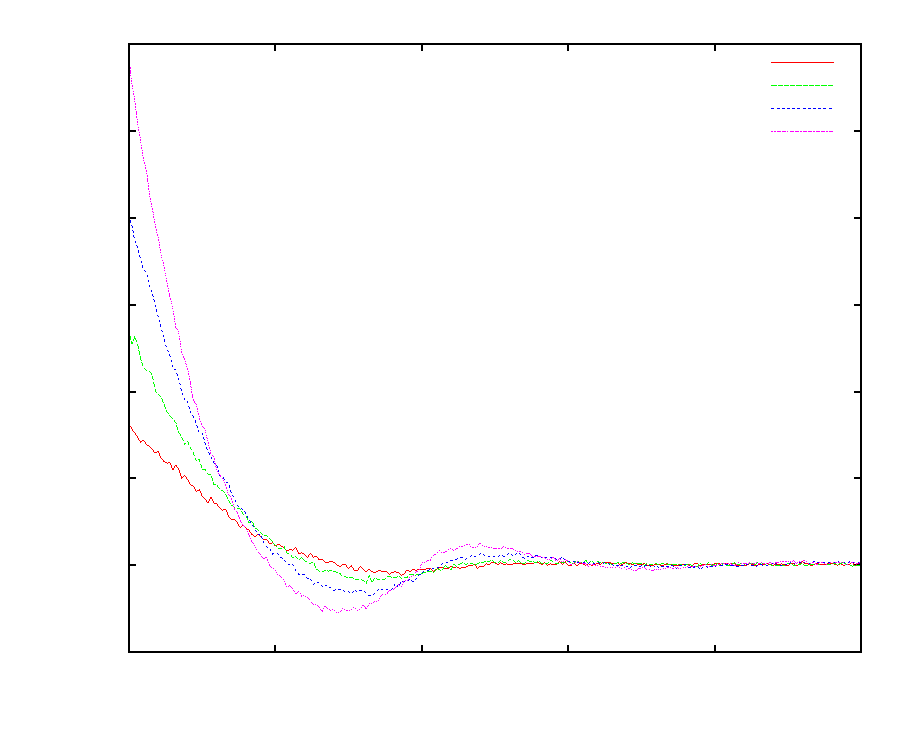
\includegraphics{PairDistribution1}}%
    \gplfronttext
  \end{picture}%
\endgroup
}
 \caption{Paarverteilungsfunktion für verschiedene Dichten $\rho$ im Bereich von 0.2 bis 0.5 (fluid)}
 \label{fig:paarverteilung1}
\end{figure} 

Harte Kugeln durchlaufen einen Phasenübergang vom flüssigen zum festen Zustand zwischen Packungsdichten von $n_f \approx 0.494$ und $n_s \approx 0.545$, was den reduzierten Dichten $\rho_f \approx 0.943$ und $\rho_s \approx 1.041$ entspricht. Anhand von Abbildungen \ref{fig:paarverteilung2} und \ref{fig:paarverteilung3} kann man diesen Phasenübergang deutlich erkennen --- die Maxima werden immer prominenter, was auf eine geordnete Kristallstruktur schließen lässt. 
 
\begin{figure}[H]
 \centering
 \resizebox{0.9\textwidth}{!}{% GNUPLOT: LaTeX picture with Postscript
\begingroup
  \makeatletter
  \providecommand\color[2][]{%
    \GenericError{(gnuplot) \space\space\space\@spaces}{%
      Package color not loaded in conjunction with
      terminal option `colourtext'%
    }{See the gnuplot documentation for explanation.%
    }{Either use 'blacktext' in gnuplot or load the package
      color.sty in LaTeX.}%
    \renewcommand\color[2][]{}%
  }%
  \providecommand\includegraphics[2][]{%
    \GenericError{(gnuplot) \space\space\space\@spaces}{%
      Package graphicx or graphics not loaded%
    }{See the gnuplot documentation for explanation.%
    }{The gnuplot epslatex terminal needs graphicx.sty or graphics.sty.}%
    \renewcommand\includegraphics[2][]{}%
  }%
  \providecommand\rotatebox[2]{#2}%
  \@ifundefined{ifGPcolor}{%
    \newif\ifGPcolor
    \GPcolortrue
  }{}%
  \@ifundefined{ifGPblacktext}{%
    \newif\ifGPblacktext
    \GPblacktextfalse
  }{}%
  % define a \g@addto@macro without @ in the name:
  \let\gplgaddtomacro\g@addto@macro
  % define empty templates for all commands taking text:
  \gdef\gplbacktext{}%
  \gdef\gplfronttext{}%
  \makeatother
  \ifGPblacktext
    % no textcolor at all
    \def\colorrgb#1{}%
    \def\colorgray#1{}%
  \else
    % gray or color?
    \ifGPcolor
      \def\colorrgb#1{\color[rgb]{#1}}%
      \def\colorgray#1{\color[gray]{#1}}%
      \expandafter\def\csname LTw\endcsname{\color{white}}%
      \expandafter\def\csname LTb\endcsname{\color{black}}%
      \expandafter\def\csname LTa\endcsname{\color{black}}%
      \expandafter\def\csname LT0\endcsname{\color[rgb]{1,0,0}}%
      \expandafter\def\csname LT1\endcsname{\color[rgb]{0,1,0}}%
      \expandafter\def\csname LT2\endcsname{\color[rgb]{0,0,1}}%
      \expandafter\def\csname LT3\endcsname{\color[rgb]{1,0,1}}%
      \expandafter\def\csname LT4\endcsname{\color[rgb]{0,1,1}}%
      \expandafter\def\csname LT5\endcsname{\color[rgb]{1,1,0}}%
      \expandafter\def\csname LT6\endcsname{\color[rgb]{0,0,0}}%
      \expandafter\def\csname LT7\endcsname{\color[rgb]{1,0.3,0}}%
      \expandafter\def\csname LT8\endcsname{\color[rgb]{0.5,0.5,0.5}}%
    \else
      % gray
      \def\colorrgb#1{\color{black}}%
      \def\colorgray#1{\color[gray]{#1}}%
      \expandafter\def\csname LTw\endcsname{\color{white}}%
      \expandafter\def\csname LTb\endcsname{\color{black}}%
      \expandafter\def\csname LTa\endcsname{\color{black}}%
      \expandafter\def\csname LT0\endcsname{\color{black}}%
      \expandafter\def\csname LT1\endcsname{\color{black}}%
      \expandafter\def\csname LT2\endcsname{\color{black}}%
      \expandafter\def\csname LT3\endcsname{\color{black}}%
      \expandafter\def\csname LT4\endcsname{\color{black}}%
      \expandafter\def\csname LT5\endcsname{\color{black}}%
      \expandafter\def\csname LT6\endcsname{\color{black}}%
      \expandafter\def\csname LT7\endcsname{\color{black}}%
      \expandafter\def\csname LT8\endcsname{\color{black}}%
    \fi
  \fi
  \setlength{\unitlength}{0.0500bp}%
  \begin{picture}(8502.00,6802.00)%
    \gplgaddtomacro\gplbacktext{%
      \csname LTb\endcsname%
      \put(946,704){\makebox(0,0)[r]{\strut{} 0.5}}%
      \put(946,1287){\makebox(0,0)[r]{\strut{} 1}}%
      \put(946,1871){\makebox(0,0)[r]{\strut{} 1.5}}%
      \put(946,2454){\makebox(0,0)[r]{\strut{} 2}}%
      \put(946,3037){\makebox(0,0)[r]{\strut{} 2.5}}%
      \put(946,3621){\makebox(0,0)[r]{\strut{} 3}}%
      \put(946,4204){\makebox(0,0)[r]{\strut{} 3.5}}%
      \put(946,4787){\makebox(0,0)[r]{\strut{} 4}}%
      \put(946,5370){\makebox(0,0)[r]{\strut{} 4.5}}%
      \put(946,5954){\makebox(0,0)[r]{\strut{} 5}}%
      \put(946,6537){\makebox(0,0)[r]{\strut{} 5.5}}%
      \put(1078,484){\makebox(0,0){\strut{} 1}}%
      \put(2483,484){\makebox(0,0){\strut{} 1.5}}%
      \put(3889,484){\makebox(0,0){\strut{} 2}}%
      \put(5294,484){\makebox(0,0){\strut{} 2.5}}%
      \put(6700,484){\makebox(0,0){\strut{} 3}}%
      \put(8105,484){\makebox(0,0){\strut{} 3.5}}%
      \put(176,3620){\rotatebox{-270}{\makebox(0,0){\strut{}$g(r)$}}}%
      \put(4591,154){\makebox(0,0){\strut{}$r [\text{m}]$}}%
    }%
    \gplgaddtomacro\gplfronttext{%
      \csname LTb\endcsname%
      \put(7118,6364){\makebox(0,0)[r]{\strut{}$\rho$ = 0.6}}%
      \csname LTb\endcsname%
      \put(7118,6144){\makebox(0,0)[r]{\strut{}$\rho$ = 0.7}}%
      \csname LTb\endcsname%
      \put(7118,5924){\makebox(0,0)[r]{\strut{}$\rho$ = 0.8}}%
      \csname LTb\endcsname%
      \put(7118,5704){\makebox(0,0)[r]{\strut{}$\rho$ = 0.9}}%
    }%
    \gplbacktext
    \put(0,0){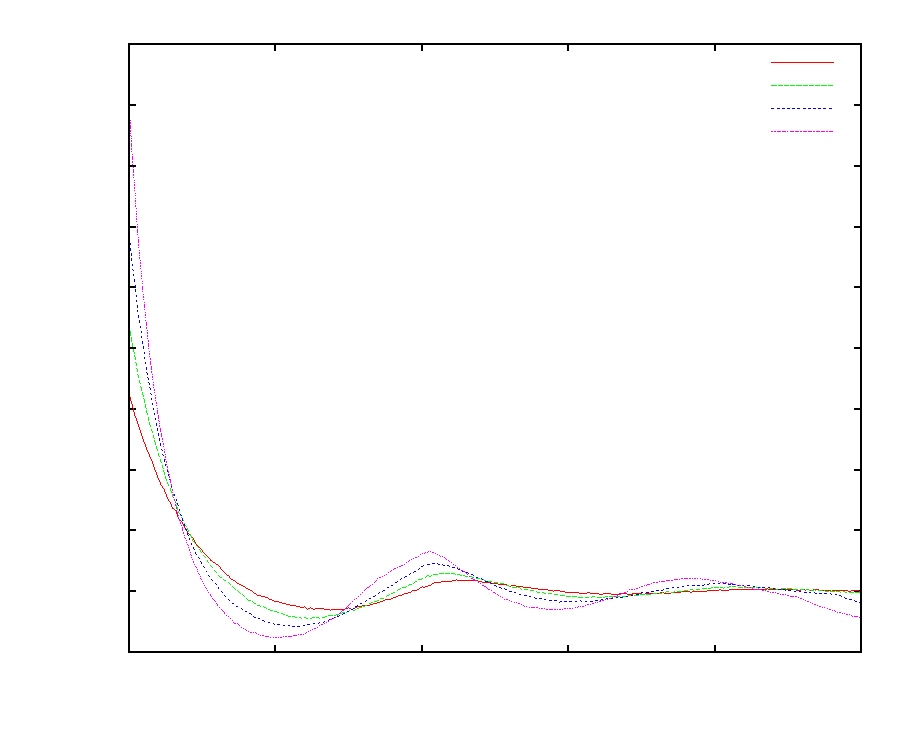
\includegraphics{PairDistribution5}}%
    \gplfronttext
  \end{picture}%
\endgroup
}
  \caption{Paarverteilungsfunktion für verschiedene Dichten $\rho$ im Bereich von 0.6 bis 0.9 (fluid) }
 \label{fig:paarverteilung2}
\end{figure} 
 
Theoretisch sollte ein System von harten Kugeln ein fcc-Kristallgitter ausbilden, dessen Gittervektoren eine relative Länge von $r_1 : r_2 : r_3 = 1 : \sqrt{2} : \sqrt{3}$ aufweisen. Bei einer Dichte von 1.3 finden sich die Maxima der Paarverteilungsfunktion auch ziemlich genau in diesen Abständen. 
 
\begin{figure}[H]
 \centering
  \resizebox{0.9\textwidth}{!}{% GNUPLOT: LaTeX picture with Postscript
\begingroup
  \makeatletter
  \providecommand\color[2][]{%
    \GenericError{(gnuplot) \space\space\space\@spaces}{%
      Package color not loaded in conjunction with
      terminal option `colourtext'%
    }{See the gnuplot documentation for explanation.%
    }{Either use 'blacktext' in gnuplot or load the package
      color.sty in LaTeX.}%
    \renewcommand\color[2][]{}%
  }%
  \providecommand\includegraphics[2][]{%
    \GenericError{(gnuplot) \space\space\space\@spaces}{%
      Package graphicx or graphics not loaded%
    }{See the gnuplot documentation for explanation.%
    }{The gnuplot epslatex terminal needs graphicx.sty or graphics.sty.}%
    \renewcommand\includegraphics[2][]{}%
  }%
  \providecommand\rotatebox[2]{#2}%
  \@ifundefined{ifGPcolor}{%
    \newif\ifGPcolor
    \GPcolortrue
  }{}%
  \@ifundefined{ifGPblacktext}{%
    \newif\ifGPblacktext
    \GPblacktextfalse
  }{}%
  % define a \g@addto@macro without @ in the name:
  \let\gplgaddtomacro\g@addto@macro
  % define empty templates for all commands taking text:
  \gdef\gplbacktext{}%
  \gdef\gplfronttext{}%
  \makeatother
  \ifGPblacktext
    % no textcolor at all
    \def\colorrgb#1{}%
    \def\colorgray#1{}%
  \else
    % gray or color?
    \ifGPcolor
      \def\colorrgb#1{\color[rgb]{#1}}%
      \def\colorgray#1{\color[gray]{#1}}%
      \expandafter\def\csname LTw\endcsname{\color{white}}%
      \expandafter\def\csname LTb\endcsname{\color{black}}%
      \expandafter\def\csname LTa\endcsname{\color{black}}%
      \expandafter\def\csname LT0\endcsname{\color[rgb]{1,0,0}}%
      \expandafter\def\csname LT1\endcsname{\color[rgb]{0,1,0}}%
      \expandafter\def\csname LT2\endcsname{\color[rgb]{0,0,1}}%
      \expandafter\def\csname LT3\endcsname{\color[rgb]{1,0,1}}%
      \expandafter\def\csname LT4\endcsname{\color[rgb]{0,1,1}}%
      \expandafter\def\csname LT5\endcsname{\color[rgb]{1,1,0}}%
      \expandafter\def\csname LT6\endcsname{\color[rgb]{0,0,0}}%
      \expandafter\def\csname LT7\endcsname{\color[rgb]{1,0.3,0}}%
      \expandafter\def\csname LT8\endcsname{\color[rgb]{0.5,0.5,0.5}}%
    \else
      % gray
      \def\colorrgb#1{\color{black}}%
      \def\colorgray#1{\color[gray]{#1}}%
      \expandafter\def\csname LTw\endcsname{\color{white}}%
      \expandafter\def\csname LTb\endcsname{\color{black}}%
      \expandafter\def\csname LTa\endcsname{\color{black}}%
      \expandafter\def\csname LT0\endcsname{\color{black}}%
      \expandafter\def\csname LT1\endcsname{\color{black}}%
      \expandafter\def\csname LT2\endcsname{\color{black}}%
      \expandafter\def\csname LT3\endcsname{\color{black}}%
      \expandafter\def\csname LT4\endcsname{\color{black}}%
      \expandafter\def\csname LT5\endcsname{\color{black}}%
      \expandafter\def\csname LT6\endcsname{\color{black}}%
      \expandafter\def\csname LT7\endcsname{\color{black}}%
      \expandafter\def\csname LT8\endcsname{\color{black}}%
    \fi
  \fi
  \setlength{\unitlength}{0.0500bp}%
  \begin{picture}(8502.00,6802.00)%
    \gplgaddtomacro\gplbacktext{%
      \csname LTb\endcsname%
      \put(814,704){\makebox(0,0)[r]{\strut{} 0}}%
      \put(814,1433){\makebox(0,0)[r]{\strut{} 2}}%
      \put(814,2162){\makebox(0,0)[r]{\strut{} 4}}%
      \put(814,2891){\makebox(0,0)[r]{\strut{} 6}}%
      \put(814,3621){\makebox(0,0)[r]{\strut{} 8}}%
      \put(814,4350){\makebox(0,0)[r]{\strut{} 10}}%
      \put(814,5079){\makebox(0,0)[r]{\strut{} 12}}%
      \put(814,5808){\makebox(0,0)[r]{\strut{} 14}}%
      \put(814,6537){\makebox(0,0)[r]{\strut{} 16}}%
      \put(946,484){\makebox(0,0){\strut{} 1}}%
      \put(2378,484){\makebox(0,0){\strut{} 1.5}}%
      \put(3810,484){\makebox(0,0){\strut{} 2}}%
      \put(5241,484){\makebox(0,0){\strut{} 2.5}}%
      \put(6673,484){\makebox(0,0){\strut{} 3}}%
      \put(8105,484){\makebox(0,0){\strut{} 3.5}}%
      \put(176,3620){\rotatebox{-270}{\makebox(0,0){\strut{}$g(r)$}}}%
      \put(4525,154){\makebox(0,0){\strut{}$r [\text{m}]$}}%
    }%
    \gplgaddtomacro\gplfronttext{%
      \csname LTb\endcsname%
      \put(7118,6364){\makebox(0,0)[r]{\strut{}$\rho$ = 1.0}}%
      \csname LTb\endcsname%
      \put(7118,6144){\makebox(0,0)[r]{\strut{}$\rho$ = 1.1}}%
      \csname LTb\endcsname%
      \put(7118,5924){\makebox(0,0)[r]{\strut{}$\rho$ = 1.2}}%
      \csname LTb\endcsname%
      \put(7118,5704){\makebox(0,0)[r]{\strut{}$\rho$ = 1.3}}%
    }%
    \gplbacktext
    \put(0,0){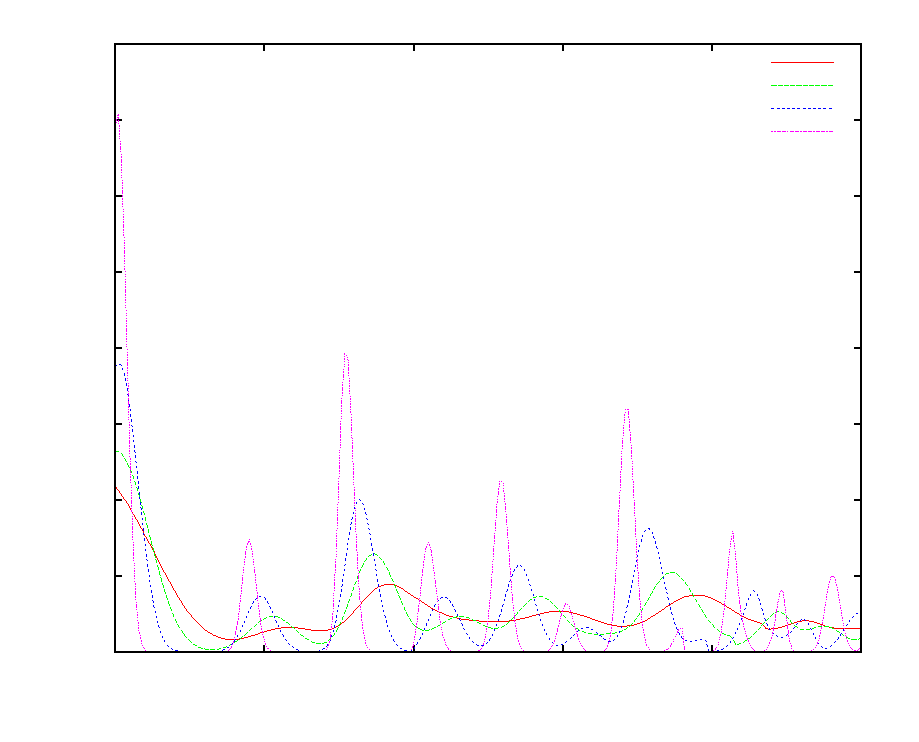
\includegraphics{PairDistribution9}}%
    \gplfronttext
  \end{picture}%
\endgroup
}
 \caption{Paarverteilungsfunktion für verschiedene Dichten $\rho$ im Bereich von 1.0 bis 1.3 (fest) }
 \label{fig:paarverteilung3}
\end{figure} 
 

\subsection{Thermische Zustandsgleichung}
Die Thermische Zustandsgleichung stellt einen Zusammenhang zwischen den Variablen Druck $p$, Temperatur $T$ und Dichte $\rho$ her. Sie kann mittels mehrerer Methoden berechnet werden. Die wohl am häufigsten verwendete bedient sich des Virials $W$  
\begin{equation}
\frac{p}{\rho k T} = 1 - \frac{1}{3NkT}\underbrace{\sum_{i=1}^N \vec{r}_i \cdot \vec{F}_i}_{= - W}
\end{equation}
Da harte Kugeln allerdings ein nicht-differenzierbares Potential besitzen und demnach keine auf sie Kraft wirkt, solange sie nicht aneinander stoßen, muss die Berechnung der Zustandsgleichung für harte Kugeln etwas abgeändert werden.

\TODO{Herleitung Zustandsgleichung über Paarverteilungsfunktion} 

\begin{equation}
\frac{p}{\rho k T} = 1 + \frac{1}{t_m} \sum_{Kollisionen} \vec{r}_{ij} \cdot \Delta \vec{v}_i
\end{equation}
wobei $\vec{r}_{ij}$ die Relativposition der beiden an der Kollision beteiligten Kugeln und $\Delta \vec{v}_i$ die Änderung der Geschwindigkeit von Kugel $i$ im Verlauf der Kollision ist.   
\begin{figure}[H]
 \centering
  \resizebox{0.9\textwidth}{!}{% GNUPLOT: LaTeX picture with Postscript
\begingroup
  \makeatletter
  \providecommand\color[2][]{%
    \GenericError{(gnuplot) \space\space\space\@spaces}{%
      Package color not loaded in conjunction with
      terminal option `colourtext'%
    }{See the gnuplot documentation for explanation.%
    }{Either use 'blacktext' in gnuplot or load the package
      color.sty in LaTeX.}%
    \renewcommand\color[2][]{}%
  }%
  \providecommand\includegraphics[2][]{%
    \GenericError{(gnuplot) \space\space\space\@spaces}{%
      Package graphicx or graphics not loaded%
    }{See the gnuplot documentation for explanation.%
    }{The gnuplot epslatex terminal needs graphicx.sty or graphics.sty.}%
    \renewcommand\includegraphics[2][]{}%
  }%
  \providecommand\rotatebox[2]{#2}%
  \@ifundefined{ifGPcolor}{%
    \newif\ifGPcolor
    \GPcolortrue
  }{}%
  \@ifundefined{ifGPblacktext}{%
    \newif\ifGPblacktext
    \GPblacktextfalse
  }{}%
  % define a \g@addto@macro without @ in the name:
  \let\gplgaddtomacro\g@addto@macro
  % define empty templates for all commands taking text:
  \gdef\gplbacktext{}%
  \gdef\gplfronttext{}%
  \makeatother
  \ifGPblacktext
    % no textcolor at all
    \def\colorrgb#1{}%
    \def\colorgray#1{}%
  \else
    % gray or color?
    \ifGPcolor
      \def\colorrgb#1{\color[rgb]{#1}}%
      \def\colorgray#1{\color[gray]{#1}}%
      \expandafter\def\csname LTw\endcsname{\color{white}}%
      \expandafter\def\csname LTb\endcsname{\color{black}}%
      \expandafter\def\csname LTa\endcsname{\color{black}}%
      \expandafter\def\csname LT0\endcsname{\color[rgb]{1,0,0}}%
      \expandafter\def\csname LT1\endcsname{\color[rgb]{0,1,0}}%
      \expandafter\def\csname LT2\endcsname{\color[rgb]{0,0,1}}%
      \expandafter\def\csname LT3\endcsname{\color[rgb]{1,0,1}}%
      \expandafter\def\csname LT4\endcsname{\color[rgb]{0,1,1}}%
      \expandafter\def\csname LT5\endcsname{\color[rgb]{1,1,0}}%
      \expandafter\def\csname LT6\endcsname{\color[rgb]{0,0,0}}%
      \expandafter\def\csname LT7\endcsname{\color[rgb]{1,0.3,0}}%
      \expandafter\def\csname LT8\endcsname{\color[rgb]{0.5,0.5,0.5}}%
    \else
      % gray
      \def\colorrgb#1{\color{black}}%
      \def\colorgray#1{\color[gray]{#1}}%
      \expandafter\def\csname LTw\endcsname{\color{white}}%
      \expandafter\def\csname LTb\endcsname{\color{black}}%
      \expandafter\def\csname LTa\endcsname{\color{black}}%
      \expandafter\def\csname LT0\endcsname{\color{black}}%
      \expandafter\def\csname LT1\endcsname{\color{black}}%
      \expandafter\def\csname LT2\endcsname{\color{black}}%
      \expandafter\def\csname LT3\endcsname{\color{black}}%
      \expandafter\def\csname LT4\endcsname{\color{black}}%
      \expandafter\def\csname LT5\endcsname{\color{black}}%
      \expandafter\def\csname LT6\endcsname{\color{black}}%
      \expandafter\def\csname LT7\endcsname{\color{black}}%
      \expandafter\def\csname LT8\endcsname{\color{black}}%
    \fi
  \fi
  \setlength{\unitlength}{0.0500bp}%
  \begin{picture}(8502.00,6802.00)%
    \gplgaddtomacro\gplbacktext{%
      \csname LTb\endcsname%
      \put(814,704){\makebox(0,0)[r]{\strut{} 0}}%
      \put(814,1676){\makebox(0,0)[r]{\strut{} 5}}%
      \put(814,2648){\makebox(0,0)[r]{\strut{} 10}}%
      \put(814,3621){\makebox(0,0)[r]{\strut{} 15}}%
      \put(814,4593){\makebox(0,0)[r]{\strut{} 20}}%
      \put(814,5565){\makebox(0,0)[r]{\strut{} 25}}%
      \put(814,6537){\makebox(0,0)[r]{\strut{} 30}}%
      \put(946,484){\makebox(0,0){\strut{} 0.2}}%
      \put(2139,484){\makebox(0,0){\strut{} 0.4}}%
      \put(3332,484){\makebox(0,0){\strut{} 0.6}}%
      \put(4526,484){\makebox(0,0){\strut{} 0.8}}%
      \put(5719,484){\makebox(0,0){\strut{} 1}}%
      \put(6912,484){\makebox(0,0){\strut{} 1.2}}%
      \put(8105,484){\makebox(0,0){\strut{} 1.4}}%
      \put(176,3620){\rotatebox{-270}{\makebox(0,0){\strut{}$p/\rho k T$}}}%
      \put(4525,154){\makebox(0,0){\strut{}$
\rho [\text{m}^{-3}]$}}%
    }%
    \gplgaddtomacro\gplfronttext{%
      \csname LTb\endcsname%
      \put(7118,6364){\makebox(0,0)[r]{\strut{}aus Paarverteilungsfunktion}}%
      \csname LTb\endcsname%
      \put(7118,6144){\makebox(0,0)[r]{\strut{}aus Impulsübertrag}}%
      \csname LTb\endcsname%
      \put(7118,5924){\makebox(0,0)[r]{\strut{}Theorie}}%
    }%
    \gplbacktext
    \put(0,0){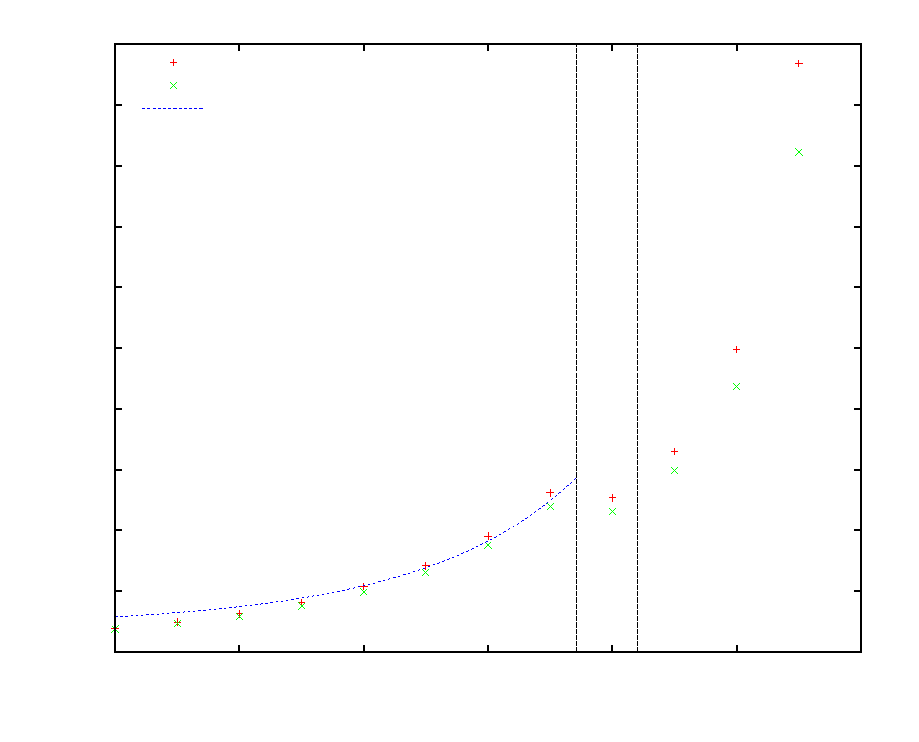
\includegraphics{eos}}%
    \gplfronttext
  \end{picture}%
\endgroup
}
 \caption{Thermische Zustandsgleichung des Systems aus harten Kugeln}
 \label{fig:zustandsgleichung}
\end{figure} 


\subsection{Diffusion}

\subsection{Collisionszeiten}